\documentclass[full]{l3doc}
\usepackage{fontspec}
\usepackage{biblatex}
\addbibresource{literatur.bib}
\newcommand{\slsh}{\textbackslash{}}
\newcommand{\TikZ}{Ti\textit{k}Z}
\def\thinmargin{\list{}{\rightmargin-50pt\leftmargin-90pt}\item[]}
\let\endthinmargin=\endlist

\usepackage{listings}
\lstset {
    basicstyle=\small\ttfamily
    ,escapeinside={+}{+}
}

\usepackage{codeanatomy}

\begin{document}

\GetFileInfo{codeanatomy.sty}
\DoNotIndex{}

\title{
  \pkg{codeanatomy} -- Draw Code Anatomy%
  \thanks{This file describes \fileversion,
    last revised \filedate.}\\[1ex]
  \normalsize{Usage}
}

\author{
 Hồng-Phúc Bùi
 \thanks{
   E-mail:
   \href{mailto:Hồng-Phúc Bùi}
     {hong-phuc.bui (at) htwsaar dot de}
  }
}

\date{Released \filedate}

\AtEndDocument{
 \printbibliography
}

\maketitle
\tableofcontents

\begin{documentation}
\section{Introduction}
The idea of this Package is to typeset illustrations of pieces of code with
annotations on each single parts of code (Code Anatomy). The origin of this idear is
code illustrations in the texbook~\autocite{sedgewick-wayne-2016}. This package
just provides tool to draw those figures.

\section{Tutorial}
In this tutorial we will draw an anatomy of a function like the
figure~\ref{fig:tut1-function} step by step.

\begin{figure}
\begin{centering}
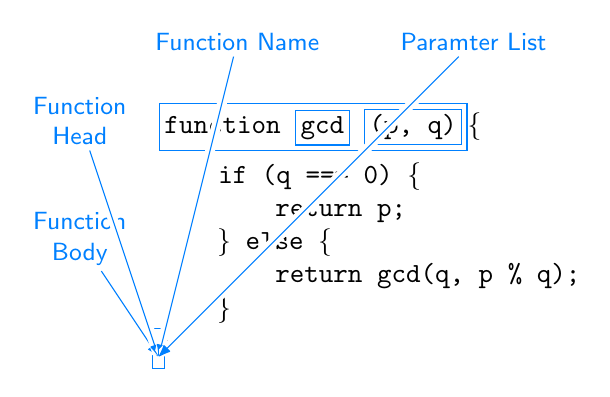
\begin{tikzpicture}[remember picture]
\codeBlock{
\cPart{functionHead}{function \cPart{functionName}{gcd} \cPart{parameterList}{(p, q)}}\{ \\[2.5pt] %
\ptab{}\mtPoint{mostLeft}if (q === 0) \{\\
\ptab\ptab{}return p; \\
\ptab{}\} else \{\\
\ptab\ptab{}return gcd(q, p \% q);\extremPoint{mostRight}\\
\ptab{}\}\mbPoint{mostBottom}\\
\}
};

\node(functionBody)[draw,code part,fit=(mostLeft) (mostRight) (mostBottom)] {};

% Anotation labels
\codeAnnotation{functionHeadText}(-1,3)  {Function\\Head}
\codeAnnotation{functionBodyText}(-1,1.5){Function\\Body}
\codeAnnotation{functionNameText}(1,4)   {Function Name}
\codeAnnotation{parameterListText} (4,4) {Paramter List}

% Annotation labels to Code
\draw[->, annotation] (functionBodyText) -- (pic cs:functionBody);
\draw[->, annotation] (functionHeadText) -- (pic cs:functionHead);
\draw[->, annotation] (functionNameText) -- (pic cs:functionName);
\draw[->, annotation] (parameterListText) -- (pic cs:parameterList);
\end{tikzpicture}

\caption{Anatomy of a function\label{fig:tut1-function}}
\end{centering}
\end{figure}

\subsection{Package Usage}
To use this package, just insert |\usepackage{codeanatomy}| in your \LaTeX{} file.

\subsection{Create an anatomy environment}
Next step is to create a |tikzpicture| environment. All commands in this package must be placed in
a |tikzpicture| environment with option |remember picture|.

\begin{thinmargin}
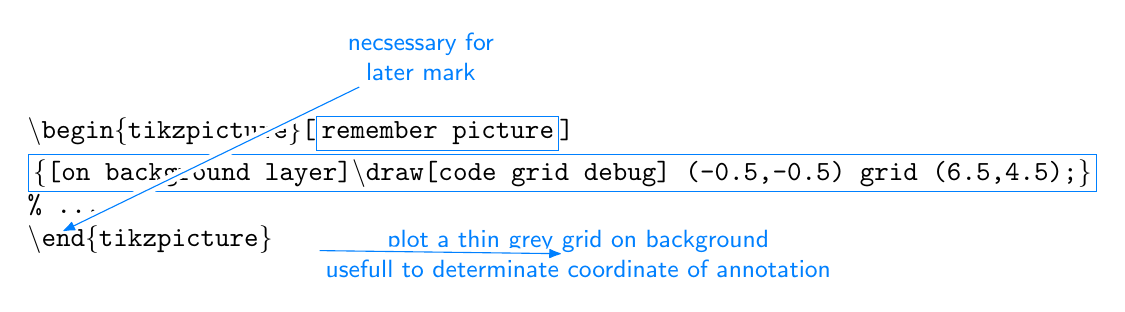
\begin{tikzpicture}[remember picture]
\codeBlock{
\textbackslash{}begin\{tikzpicture\}[\cPart{option}{remember picture}]\\
\cPart{debugGrid}{\{[on background layer]\textbackslash{}draw[code grid debug] (-0.5,-0.5) grid (6.5,4.5);\}}\\
\% ... \\
\textbackslash{}end\{tikzpicture\}
}

% Annotation labels
\codeAnnotation{optionText}    (5,2.5) {necsessary for\\later mark}
\codeAnnotation{debugGridText} (7,0)   {plot a thin grey grid on background\\usefull to determinate coordinate of annotation}

% Annotation labels to code
\draw[->, annotation] (optionText) -- (option);
\draw[->, annotation] (debugGridText) -- (debugGrid);
\end{tikzpicture}
\end{thinmargin}


\subsection{Typeset Code Listing in a TikZ-Node}
As next step we need to put the piece of code in the |tikzpicture| environment using
the command |\codeBlock|. \medskip


\begin{thinmargin}
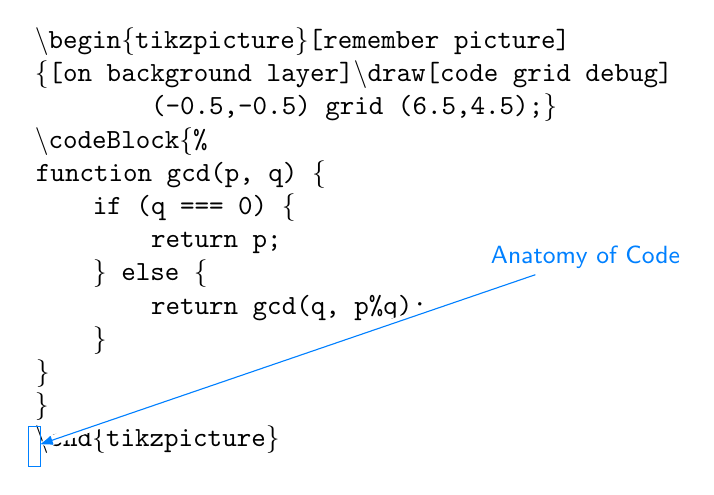
\begin{tikzpicture}[remember picture]
\codeBlock{
\textbackslash{}begin\{tikzpicture\}[remember picture]\\
\{[on background layer]\textbackslash{}draw[code grid debug]\\
                       \ptab\ptab (-0.5,-0.5) grid (6.5,4.5);\}\\
\textbackslash{}codeBlock\{\% \\
\mtPoint{mostLeft}function gcd(p, q) \{ \\
\ptab{}if (q === 0) \{ \\
\ptab\ptab{}return p; \\
\ptab{}\} else \{ \\
\ptab\ptab{}return gcd(q, p\%q);\extremPoint{mostRight}\\
\ptab\} \\
\mbPoint{mostBottom}\}\\
\} \\
\textbackslash{}end\{tikzpicture\}
}

\node(codeBlockBody)[draw,code part,fit=(mostLeft) (mostRight) (mostBottom)] {};

\codeAnnotation{codeBlockBodyText} (7,2.5) {Anatomy of Code}
\draw[->, annotation] (codeBlockBodyText) -- (codeBlockBody);
\end{tikzpicture}
\end{thinmargin}

The result of the above code is shown in the figure~\ref{fig:function-compressed},
which is not what we really want. All extra whitespaces and newlines in the
listing are removed, further more |{| and |}| are interpreted as \LaTeX{} tokens and are not
displayed.

\begin{figure}[h]
\begin{centering}
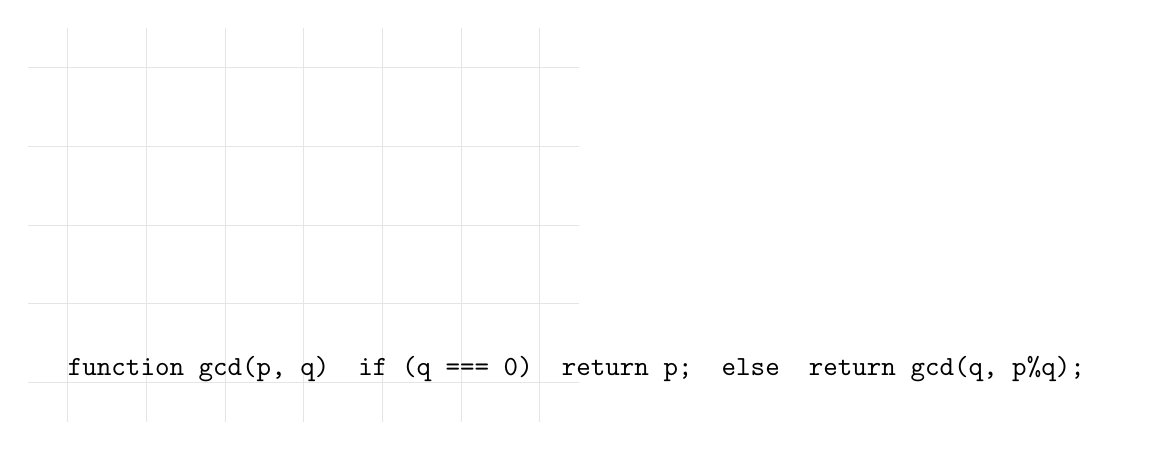
\begin{tikzpicture}[remember picture]
{[on background layer]\draw[code grid debug] (-0.5,-0.5) grid (6.5,4.5);}
\codeBlock{
function gcd(p, q) {
    if (q === 0) {
        return p;
    } else {
        return gcd(q, p\%q);
    }
}
}
\end{tikzpicture}
\caption{Unformated Code\label{fig:function-compressed}}
\end{centering}
\end{figure}


We need to put |\ptab| and |\\| into code to keep whitespaces and newlines. The characters |{| and |}|
also need to be escaped by prefixing a |\| before them.

\begin{thinmargin}
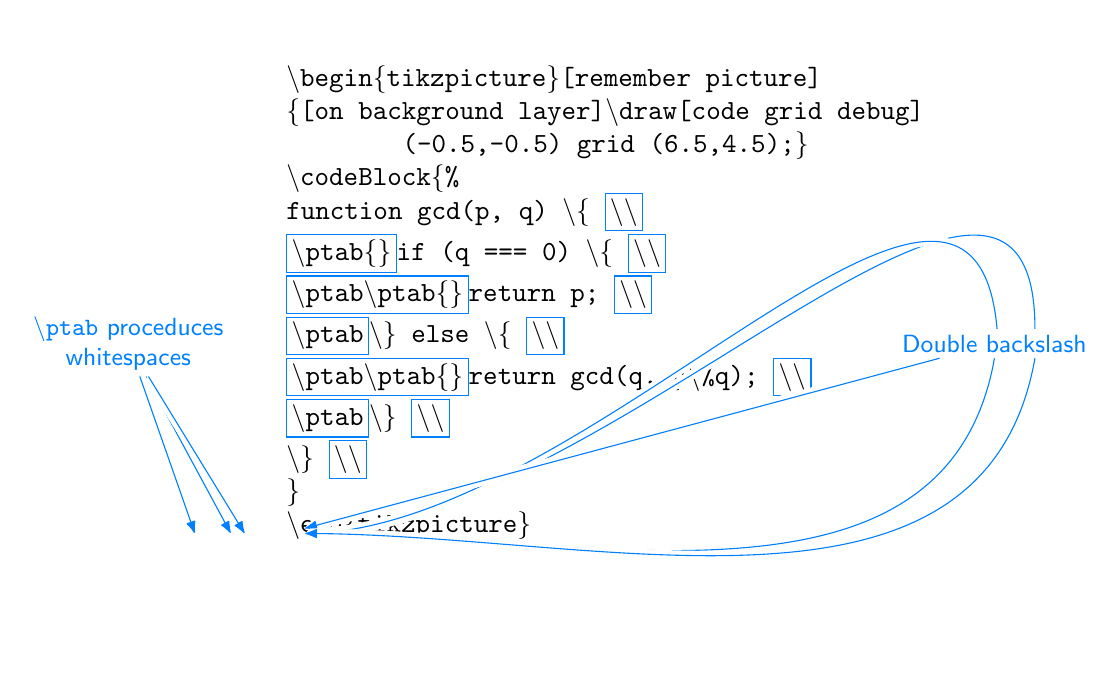
\begin{tikzpicture}[remember picture]
\codeBlock{
\textbackslash{}begin\{tikzpicture\}[remember picture]\\
\{[on background layer]\textbackslash{}draw[code grid debug]\\
                       \ptab\ptab (-0.5,-0.5) grid (6.5,4.5);\}\\
\textbackslash{}codeBlock\{\%\\
function gcd(p, q) \slsh\{                          \cPart{sh1}{\slsh\slsh}\\
\cPart{ptab1}{\slsh{}ptab\{\}}if (q === 0) \slsh\{                 \cPart{sh2}{\slsh\slsh}\\
\cPart{ptab2}{\slsh{}ptab\slsh{}ptab\{\}}return p;                 \cPart{sh3}{\slsh\slsh}\\
\cPart{ptab3}{\slsh{}ptab}\slsh\} else \slsh\{                     \cPart{sh4}{\slsh\slsh}\\
\cPart{ptab4}{\slsh{}ptab\slsh{}ptab\{\}}return gcd(q, p\slsh\%q); \cPart{sh5}{\slsh\slsh}\\
\cPart{ptab5}{\slsh{}ptab}\slsh\}                                  \cPart{sh6}{\slsh\slsh}\\
\slsh\}                                             \cPart{sh7}{\slsh\slsh}\\
\} \\
\textbackslash{}end\{tikzpicture\}
}

% Annotation labels
\codeAnnotation{shText}    (9,2.5) {Double backslash}
\codeAnnotation{ptabText}  (-2,2.5) {\texttt{\slsh{}ptab} proceduces\\whitespaces}
% Annotation labels to code
\draw[->, annotation] (shText.20) to[out=90,in=0] (sh1.east);
\draw[->, annotation] (shText.80) to[out=95,in=0] (sh2.east);
\draw[->, annotation] (shText) -- (sh3);
\draw[->, annotation] (shText) -- (sh4);
\draw[->, annotation] (shText) -- (sh5);
\draw[->, annotation] (shText.270) to[out=260,in=0] (sh6);
\draw[->, annotation] (shText.340) to[out=260,in=0] (sh7);

\draw[->, annotation] (ptabText) -- (ptab1.west);
\draw[->, annotation] (ptabText) -- (ptab2.west);
\draw[->, annotation] (ptabText) -- (ptab3.west);
\draw[->, annotation] (ptabText) -- (ptab4.west);
\draw[->, annotation] (ptabText) -- (ptab5.west);
\end{tikzpicture}
\end{thinmargin}

The result (figure~\ref{fig:function-formated}) is much more like what we expect
than the version before (figure~\ref{fig:function-compressed}).

\begin{figure}[h]
\begin{centering}
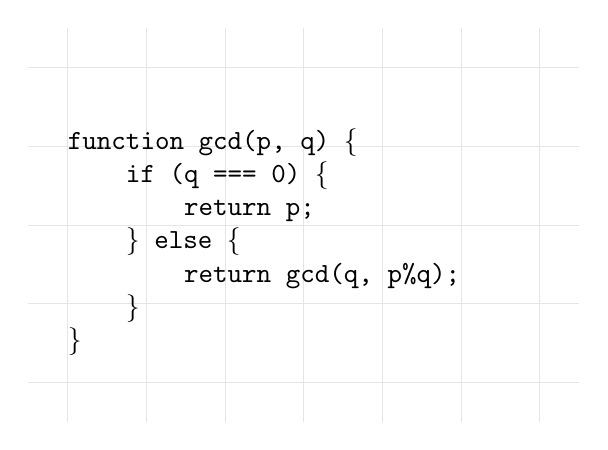
\begin{tikzpicture}[remember picture]
{[on background layer]\draw[code grid debug] (-0.5,-0.5) grid (6.5,4.5);}
\codeBlock{
function gcd(p, q) \{ \\
\ptab{}if (q === 0) \{ \\
\ptab\ptab{}return p; \\
\ptab\} else \{ \\
\ptab\ptab{}return gcd(q, p\%q); \\
\ptab\} \\
\} \\
}
\end{tikzpicture}
\caption{Formated Function\label{fig:function-formated}}
\end{centering}
\end{figure}

\subsection{Mark Parts of Code}
Now we can mark interesting parts of code with a blue boxes created by |\cPart|. At some positions
we can use |\\[<length>]| to add a little amount of vertical space, sothat the boxes do not touch
each others.

\begin{thinmargin}
{\footnotesize
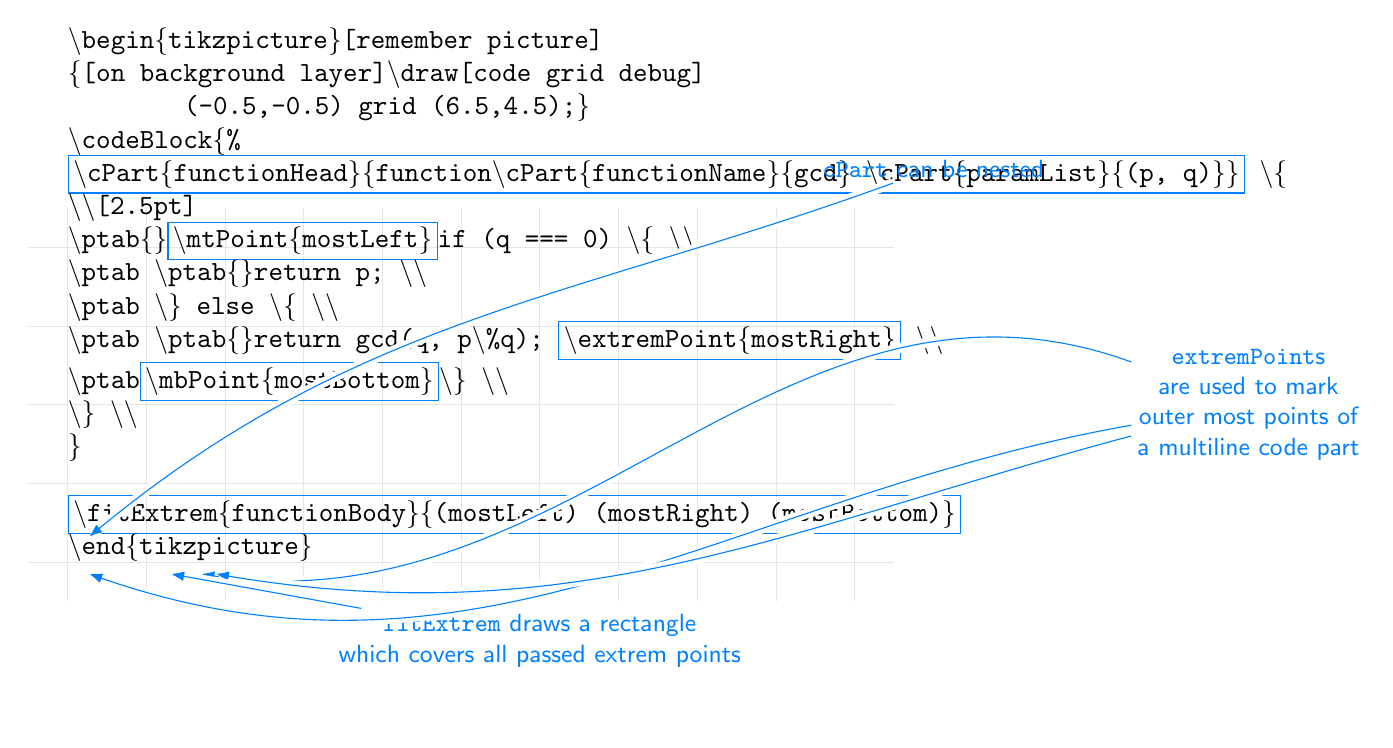
\begin{tikzpicture}[remember picture]
{[on background layer]\draw[code grid debug] (-0.5,-0.5) grid (10.5,4.5);}\\
\codeBlock{
\textbackslash{}begin\{tikzpicture\}[remember picture]\\
\{[on background layer]\textbackslash{}draw[code grid debug]\\
                       \ptab\ptab (-0.5,-0.5) grid (6.5,4.5);\}\\
\textbackslash{}codeBlock\{\%\\
\cPart{nestedCodePart}{\slsh{}cPart\{functionHead\}\{function\slsh{}cPart\{functionName\}\{gcd\} \slsh{}cPart\{paramList\}\{(p, q)\}\}} \slsh\{\\
  \slsh\slsh[2.5pt]\\
\slsh{}ptab\{\}\cPart{ep1}{\slsh{}mtPoint\{mostLeft\}}if (q === 0) \slsh\{                                                         \slsh\slsh\\
\slsh{}ptab                                               \slsh{}ptab\{\}return p;                                                               \slsh\slsh\\
\slsh{}ptab                                                   \slsh\} else \slsh\{                                                               \slsh\slsh\\
\slsh{}ptab                                               \slsh{}ptab\{\}return gcd(q, p\slsh\%q); \cPart{ep2}{\slsh{}extremPoint\{mostRight\}}  \slsh\slsh\\
\slsh{}ptab\cPart{ep3}{\slsh{}mbPoint\{mostBottom\}}\slsh\}                                                                     \slsh\slsh\\
\slsh\}                                                                                                                                          \slsh\slsh\\
\} \\
   \\
\cPart{fitExtemCmd}{\slsh{}fitExtrem\{functionBody\}\{(mostLeft) (mostRight) (mostBottom)\}}\\
\slsh{}end\{tikzpicture\}
}

\codeAnnotation{nestedCodePartText}(11,5){\texttt{cPart} can be nested}
\codeAnnotation{exText}            (15,2){\texttt{extremPoint}s\\are used to mark\\outer most points of\\a multiline code part}
\codeAnnotation{fitExtemCmdText}   (6,-1){\texttt{fitExtrem} draws a rectangle\\which covers all passed extrem points}

\draw[->, annotation] (nestedCodePartText) to[out=200,in=40] (nestedCodePart);
\draw[->, annotation] (exText) to[out=160,in=350] (ep1.south east);
\draw[->, annotation] (exText) to[out=190,in=340] (ep2.320);
\draw[->, annotation] (exText) to[out=195,in=350] (ep3.south east);
\draw[->, annotation] (fitExtemCmdText) -- (fitExtemCmd);
\end{tikzpicture}
}
\end{thinmargin}


\begin{figure}[ht]
\centering
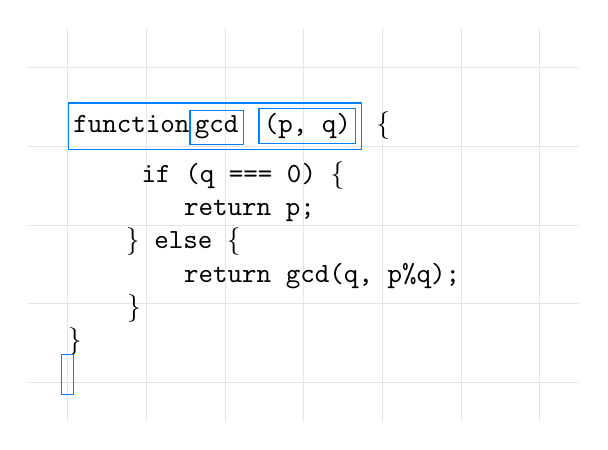
\begin{tikzpicture}[remember picture]
{[on background layer]\draw[code grid debug]
    (-0.5,-0.5) grid (6.5,4.5);}
\codeBlock{%
\cPart{functionHead}{function\cPart{functionName}{gcd} \cPart{paramList}{(p, q)}} \{
\\[2.5pt]
\ptab{}\mtPoint{mostLeft} if (q === 0) \{ \\
\ptab\ptab{}return p; \\
\ptab\} else \{ \\
\ptab\ptab{}return gcd(q, p\%q); \extremPoint{mostRight} \\
\ptab\mbPoint{mostBottom}\} \\
\} \\
}
\fitExtrem{functionBody}{(mostLeft) (mostRight) (mostBottom)}
\end{tikzpicture}
\caption{Function with marked parts\label{fig:function-parts}}
\end{figure}

\subsection{Create Annotation Labels}
We can use |\codeAnnotation| to create annotation labels for each parts of code. To draw an
arrow from label to a code part we can use the \TikZ{}command\\
|\draw[->,annotation]| \parg{annotation label} |--| \parg{code part} |;|.\\
Whereas \parg{annotation label}s are the first argument of |\codeAnnotation|s and
\parg{code part}s are the first argument of |\cPart|s.

\begin{thinmargin}
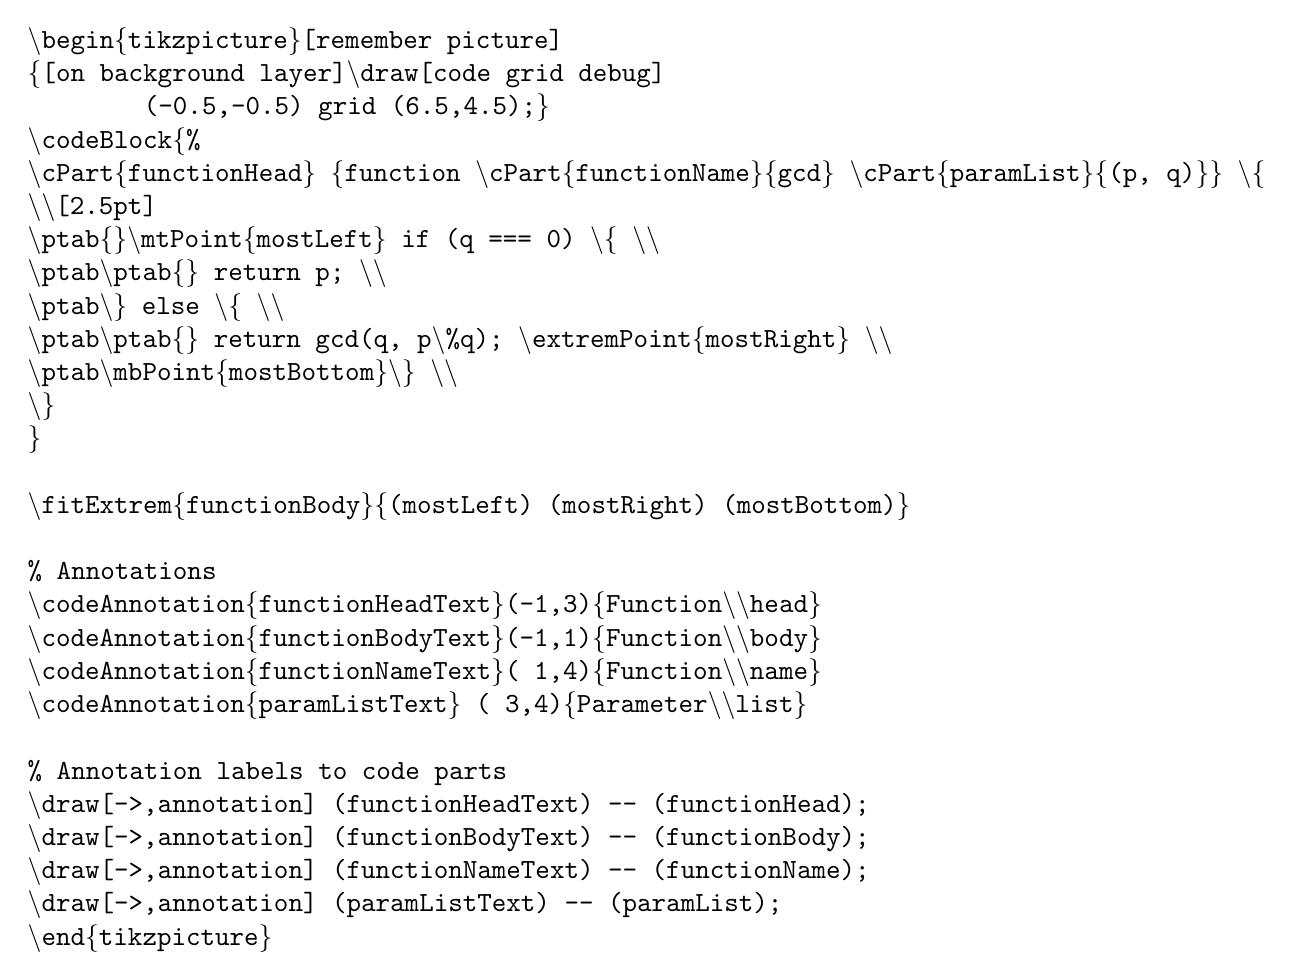
\begin{tikzpicture}[remember picture]
\codeBlock{
\textbackslash{}begin\{tikzpicture\}[remember picture]\\
\{[on background layer]\textbackslash{}draw[code grid debug]\\
                       \ptab\ptab (-0.5,-0.5) grid (6.5,4.5);\}\\
\textbackslash{}codeBlock\{\%\\
\slsh{}cPart\{functionHead\}                \{function \slsh{}cPart\{functionName\}\{gcd\} \slsh{}cPart\{paramList\}\{(p, q)\}\} \slsh\{\\
  \slsh\slsh[2.5pt]\\
\slsh{}ptab\{\}\slsh{}mtPoint\{mostLeft\}        if (q === 0) \slsh\{                                                                                \slsh\slsh\\
\slsh{}ptab\slsh{}ptab\{\}                           return p;                                                                                       \slsh\slsh\\
\slsh{}ptab\slsh                                 \} else \slsh\{                                                                                     \slsh\slsh\\
\slsh{}ptab\slsh{}ptab\{\}                           return gcd(q, p\slsh\%q);       \slsh{}extremPoint\{mostRight\}                                 \slsh\slsh\\
\slsh{}ptab\slsh{}mbPoint\{mostBottom\}\slsh\}                                                                                                      \slsh\slsh\\
\slsh\}                                             \\
\} \\
   \\
\slsh{}fitExtrem\{functionBody\}\{(mostLeft) (mostRight) (mostBottom)\}\\
\\
\% Annotations \\
\slsh{}codeAnnotation\{functionHeadText\}(-1,3)\{Function\slsh\slsh{}head\} \\
\slsh{}codeAnnotation\{functionBodyText\}(-1,1)\{Function\slsh\slsh{}body\} \\
\slsh{}codeAnnotation\{functionNameText\}( 1,4)\{Function\slsh\slsh{}name\} \\
\slsh{}codeAnnotation\{paramListText\}   ( 3,4)\{Parameter\slsh\slsh{}list\} \\
\\
\% Annotation labels to code parts\\
\slsh{}draw[->,annotation] (functionHeadText) -- (functionHead);\\
\slsh{}draw[->,annotation] (functionBodyText) -- (functionBody);\\
\slsh{}draw[->,annotation] (functionNameText) -- (functionName);\\
\slsh{}draw[->,annotation] (paramListText) -- (paramList);\\
\slsh{}end\{tikzpicture\}
}

\end{tikzpicture}
\end{thinmargin}

Instead of operator |--| we can use operator |to| \oarg{\TikZ{} options} to draw a path from
\parg{annotation label} to \parg{code part}. Finally we can remove the command
|\draw[code grid debug]...| at the begin of the |tikzpicture|.
The final result is shown in the figure~\ref{fig:function-final}, which is almost the same
as figure~\ref{fig:tut1-function}.

\begin{figure}[ht]
\centering
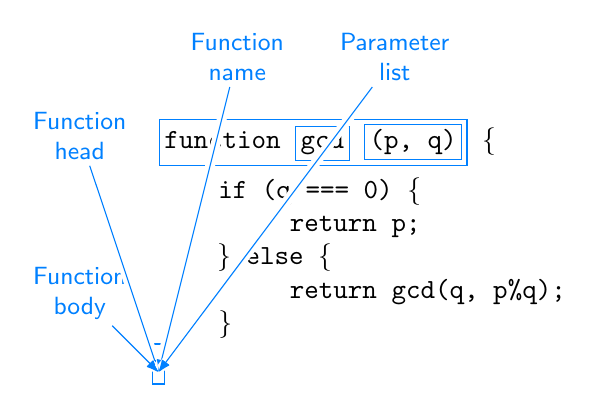
\begin{tikzpicture}[remember picture]
\codeBlock{%
\cPart{functionHead} {function \cPart{functionName}{gcd} \cPart{paramList}{(p, q)}} \{
\\[2.5pt]
\ptab{}\mtPoint{mostLeft}if (q === 0) \{ \\
\ptab\ptab{} return p; \\
\ptab\} else \{ \\
\ptab\ptab{} return gcd(q, p\%q);\extremPoint{mostRight} \\
\ptab\mbPoint{mostBottom}\} \\
\}
}
\fitExtrem{functionBody}{(mostLeft) (mostRight) (mostBottom)}
% Annotations
\codeAnnotation{functionHeadText}(-1,3){Function\\head}
\codeAnnotation{functionBodyText}(-1,1){Function\\body}
\codeAnnotation{functionNameText}( 1,4){Function\\name}
\codeAnnotation{paramListText} ( 3,4){Parameter\\list}
% Annotation labels to code parts
\draw[->,annotation] (functionHeadText)  -- (pic cs:functionHead);
\draw[->,annotation] (functionBodyText)  -- (pic cs:functionBody);
\draw[->,annotation] (functionNameText)  -- (pic cs:functionName);
\draw[->,annotation] (paramListText) --  (pic cs:paramList);
\end{tikzpicture}

\caption{Function with Annotation Labels\label{fig:function-final}}
\end{figure}

\section{Usage in conjuntion with \pkg{listings}}

As we see in the previous section, the command |\codeBlock| cannot typeset whitespaces correctly as we
expect. A way to typeset code listing is using the package \pkg{listings}. See \texttt{codeanatomy.lstlisting.pdf}
for more information.

\section{Customize style}

\changes{v0.4-Beta}
        {2023/01/24}
        {Add Option \oarg{style} to \texttt{cPart} and \texttt{iPart}}

Maybe we want to highlight the function name \texttt{gcd} with some background color like
figure~\ref{fig:function-with-highlight}. The best way to do this task is to assign this
highlight format to a \TikZ{} style --e.g. \texttt{jsid}-- and apply the style to the highlighted nodes. So they
have the same format.


% output the anatomy
\begin{figure}[htpb]
\centering
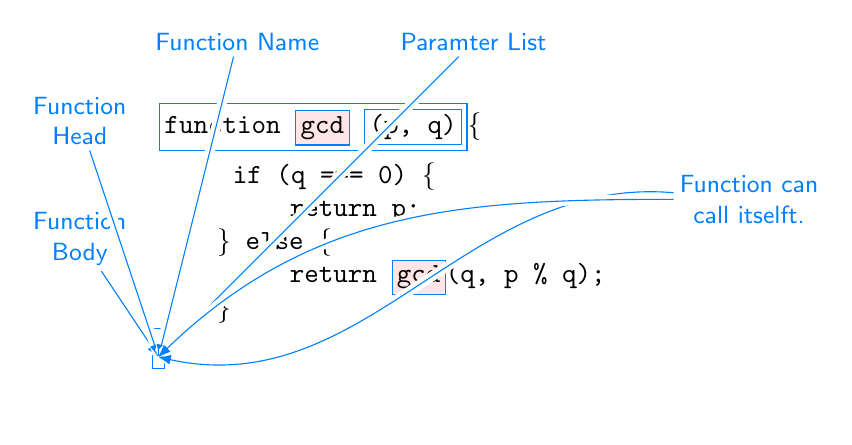
\begin{tikzpicture}[remember picture]
\tikzstyle{jsid} = [code part, fill=red!10]
%{[on background layer]\draw[code grid debug](-0.5,-0.5) grid (9.5,4.5);}
\codeBlock{
\cPart{functionHead}{function \cPart[jsid]{functionName}{gcd} \cPart{parameterList}{(p, q)}}\{ \\[2.5pt] %
\ptab{}\mtPoint{mostLeft} if (q === 0) \{\\
\ptab\ptab{} return p; \\
\ptab{}\} else \{\\
\ptab\ptab{} return \cPart[jsid]{recursive}{gcd}(q, p \% q);\extremPoint{mostRight}\\
\ptab{}\}\mbPoint{mostBottom}\\
\}
}

\fitExtrem{functionBody}{ (mostLeft) (mostRight) (mostBottom) };

% Anotation labels
\codeAnnotation{functionHeadText}(-1,3)  {Function\\Head}
\codeAnnotation{functionBodyText}(-1,1.5){Function\\Body}
\codeAnnotation{functionNameText} (1,4)  {Function Name}
\codeAnnotation{parameterListText}(4,4) {Paramter List}

\codeAnnotation{recursiveText} (7.5,2) {Function can\\call itselft.}

% Annotation labels to Code
\draw[->, annotation] (functionBodyText) -- (pic cs:functionBody);
\draw[->, annotation] (functionHeadText) -- (pic cs:functionHead);
\draw[->, annotation] (functionNameText) -- (pic cs:functionName);
\draw[->, annotation] (parameterListText) -- (pic cs:parameterList);

\draw[->, annotation] (recursiveText) to[out=175,in=-15] (pic cs:functionName);
\draw[->, annotation] (recursiveText) to[out=180,in=45]  (pic cs:recursive.north east);

\end{tikzpicture}
\caption{Highlighted name of the function\label{fig:function-with-highlight}}
\end{figure}


%out the Source code

\begin{thinmargin}
{\footnotesize
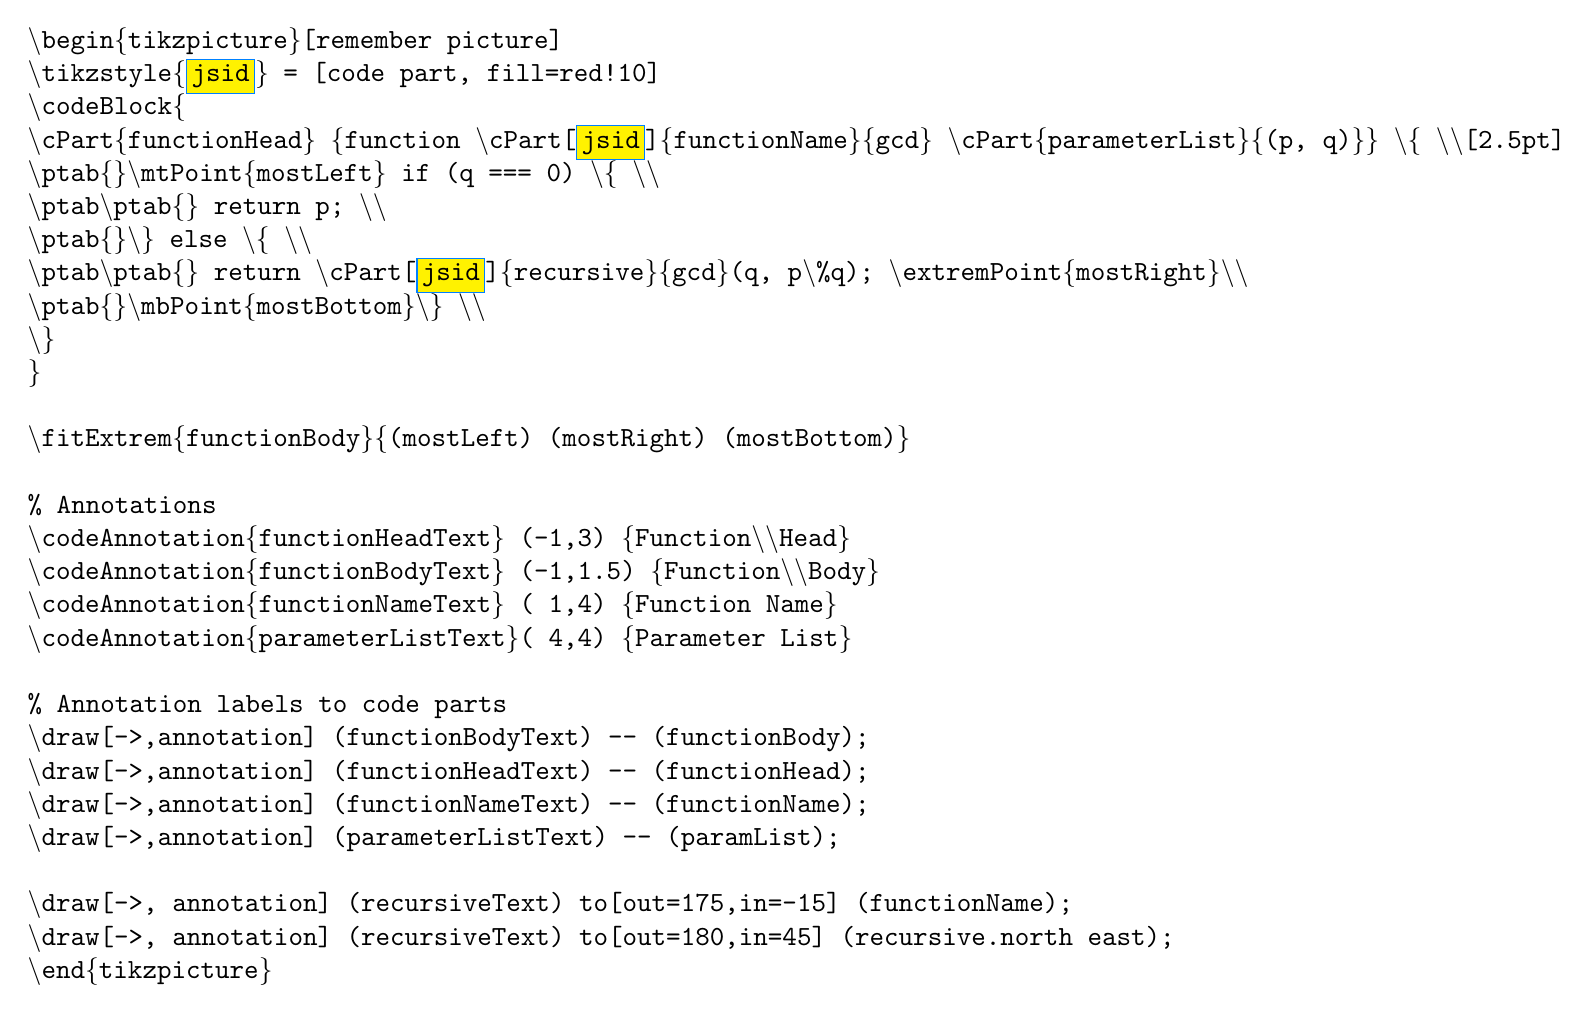
\begin{tikzpicture}[remember picture]
\tikzstyle{smark} = [code part, fill=yellow]
\codeBlock{
\textbackslash{}begin\{tikzpicture\}[remember picture]\\
\slsh{}tikzstyle\{\cPart[smark]{defstyle}{jsid}\} = [code part, fill=red!10]\\
\slsh{}codeBlock\{\\
\slsh{}cPart\{functionHead\}                \{function \slsh{}cPart[\cPart[smark]{u1}{jsid}]\{functionName\}\{gcd\} \slsh{}cPart\{parameterList\}\{(p, q)\}\} \slsh\{  \slsh\slsh[2.5pt]\\
\slsh{}ptab\{\}\slsh{}mtPoint\{mostLeft\}        if (q === 0) \slsh\{                                                                           \slsh\slsh\\
\slsh{}ptab\slsh{}ptab\{\}                           return p;                                                                                  \slsh\slsh\\
\slsh{}ptab\{\}\slsh                            \} else \slsh\{                                                                                \slsh\slsh\\
\slsh{}ptab\slsh{}ptab\{\}                           return \slsh{}cPart[\cPart[smark]{u2}{jsid}]\{recursive\}\{gcd\}(q, p\slsh\%q);       \slsh{}extremPoint\{mostRight\}\slsh\slsh\\
\slsh{}ptab\{\}\slsh{}mbPoint\{mostBottom\}\slsh\}                                                                                                  \slsh\slsh\\
\slsh\}                                             \\
\} \\
   \\
\slsh{}fitExtrem\{functionBody\}\{(mostLeft) (mostRight) (mostBottom)\}\\
\\
\% Annotations \\
\slsh{}codeAnnotation\{functionHeadText\} (-1,3)   \{Function\slsh\slsh{}Head\} \\
\slsh{}codeAnnotation\{functionBodyText\} (-1,1.5) \{Function\slsh\slsh{}Body\} \\
\slsh{}codeAnnotation\{functionNameText\} ( 1,4)   \{Function Name\} \\
\slsh{}codeAnnotation\{parameterListText\}( 4,4)   \{Parameter List\} \\
\\
\% Annotation labels to code parts\\
\slsh{}draw[->,annotation] (functionBodyText) -- (functionBody);\\
\slsh{}draw[->,annotation] (functionHeadText) -- (functionHead);\\
\slsh{}draw[->,annotation] (functionNameText) -- (functionName);\\
\slsh{}draw[->,annotation] (parameterListText) -- (paramList);\\
\\
\slsh{}draw[->, annotation] (recursiveText) to[out=175,in=-15] (functionName);\\
\slsh{}draw[->, annotation] (recursiveText) to[out=180,in=45] (recursive.north east);\\
\slsh{}end\{tikzpicture\}
}
\end{tikzpicture}
}
\end{thinmargin}

\PrintChanges
\end{documentation}
\end{document}

